\subsection{Unfolded Distributions}
\label{sec:gbb-results}

Figure~\ref{fig:gbb-results} presents a summary of the results.

\begin{figure}[htpb!]
\begin{center}
  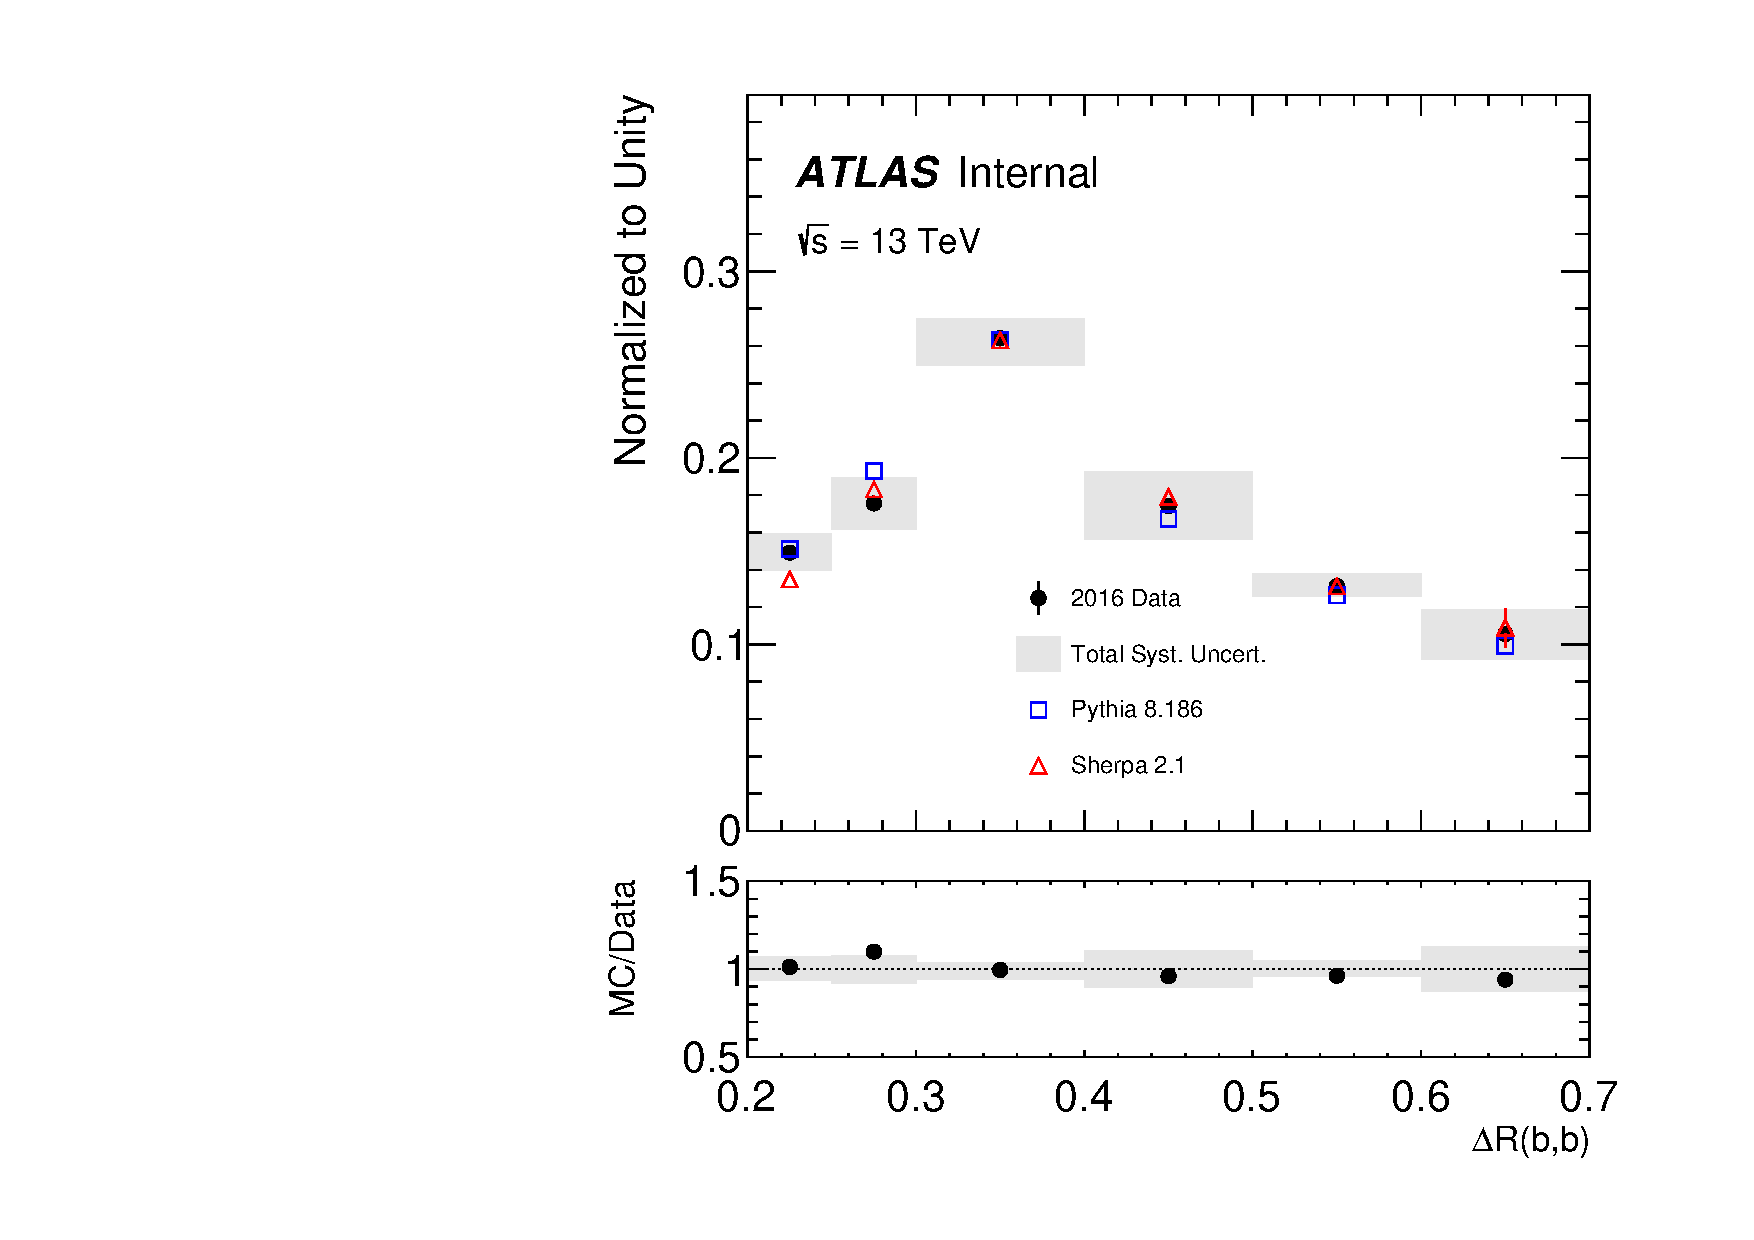
\includegraphics[width=0.45\linewidth]{figures/gbb/Unfolding/dR_unfolded_data.pdf}
  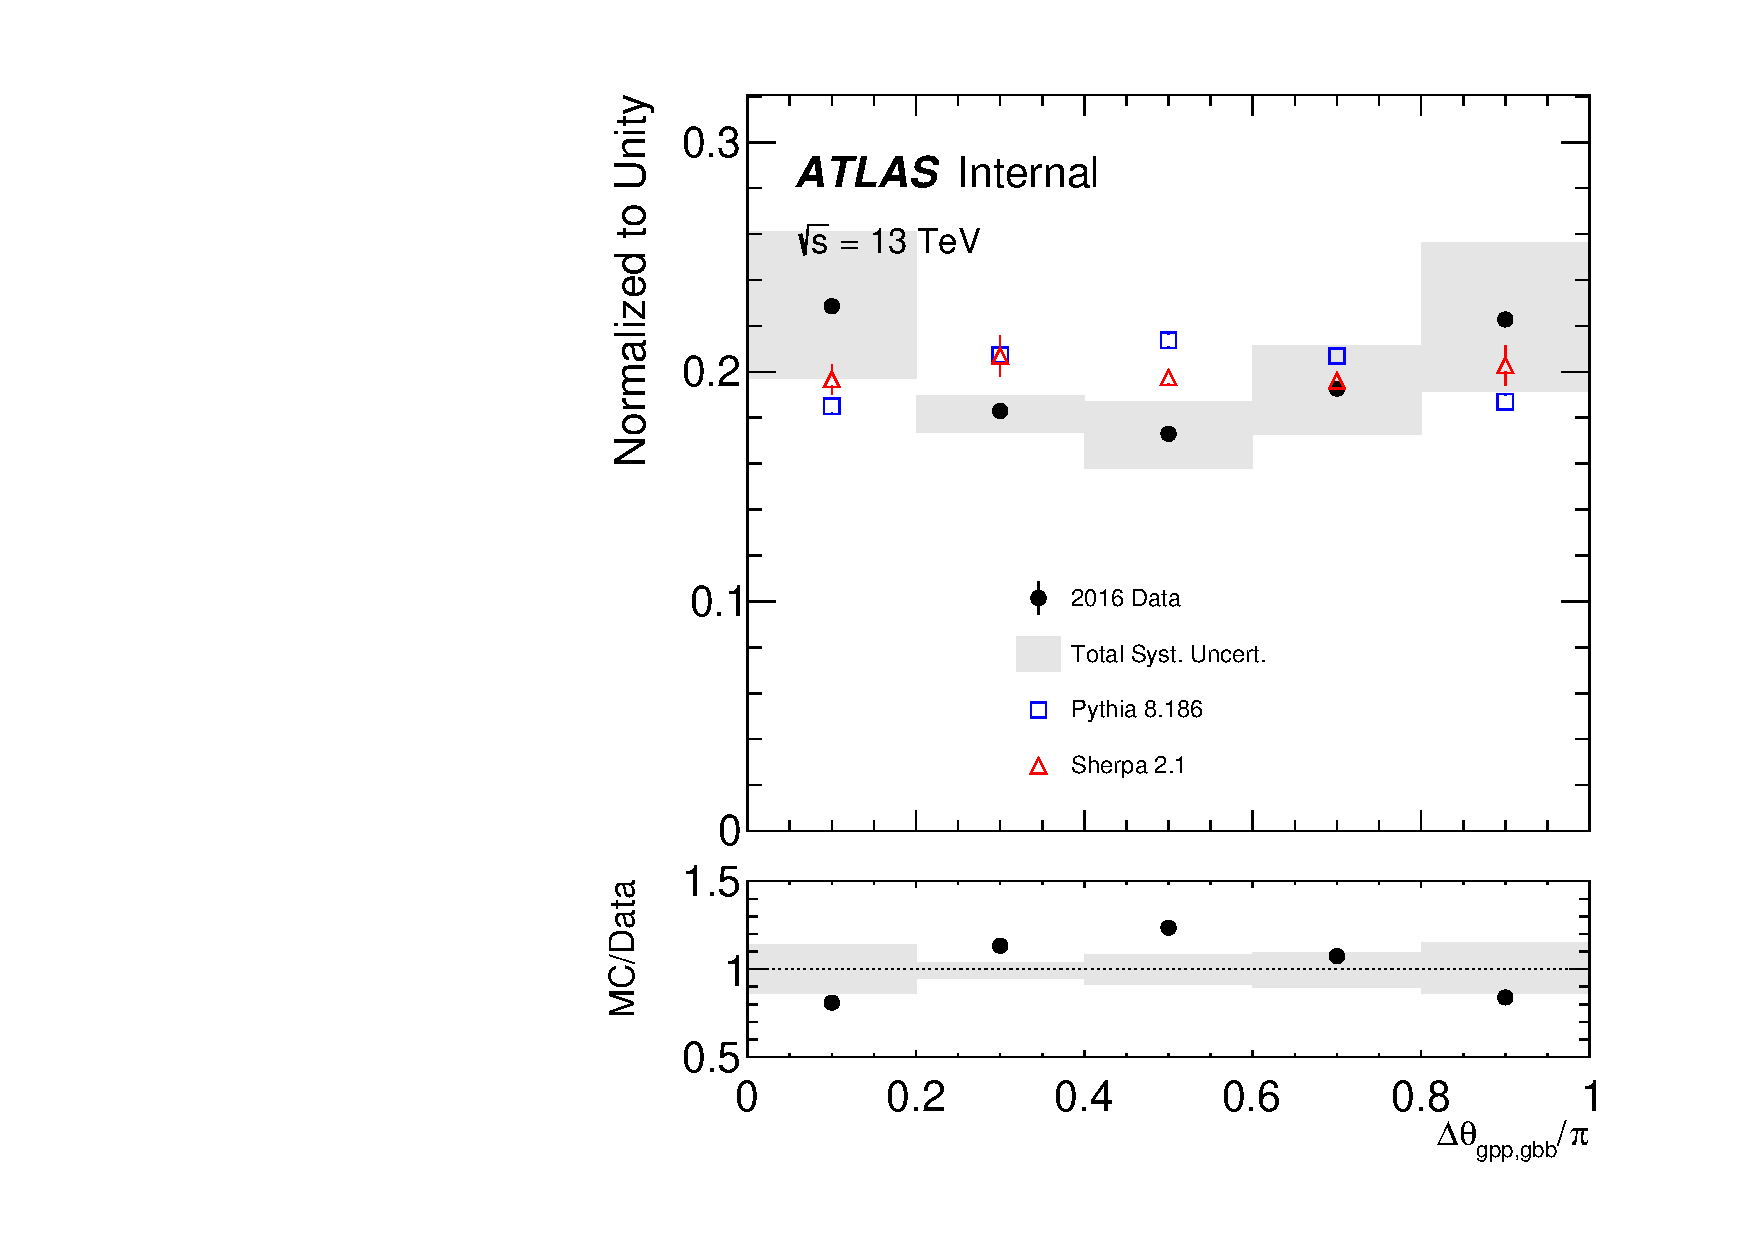
\includegraphics[width=0.45\linewidth]{figures/gbb/Unfolding/dphi_unfolded_data.pdf}\\
  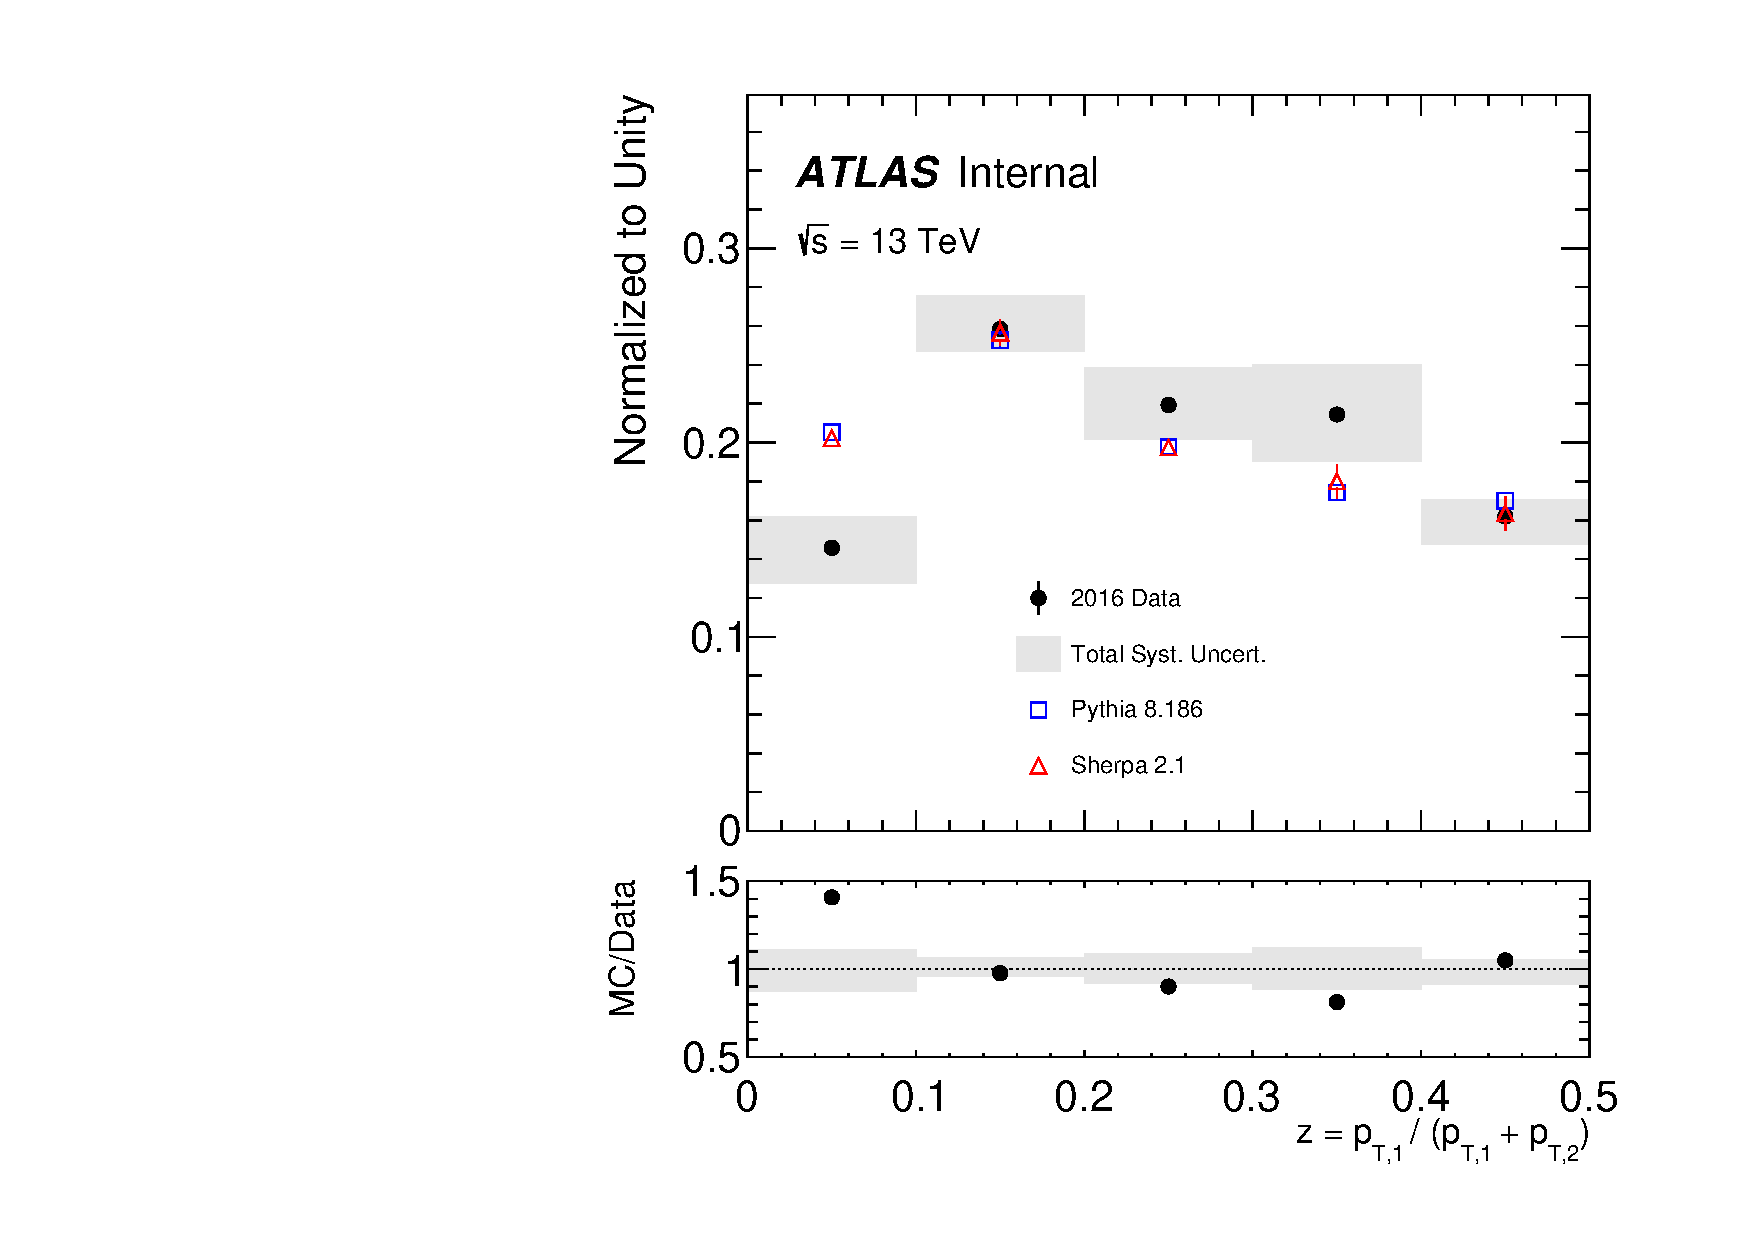
\includegraphics[width=0.45\linewidth]{figures/gbb/Unfolding/ZpT_unfolded_data.pdf}
  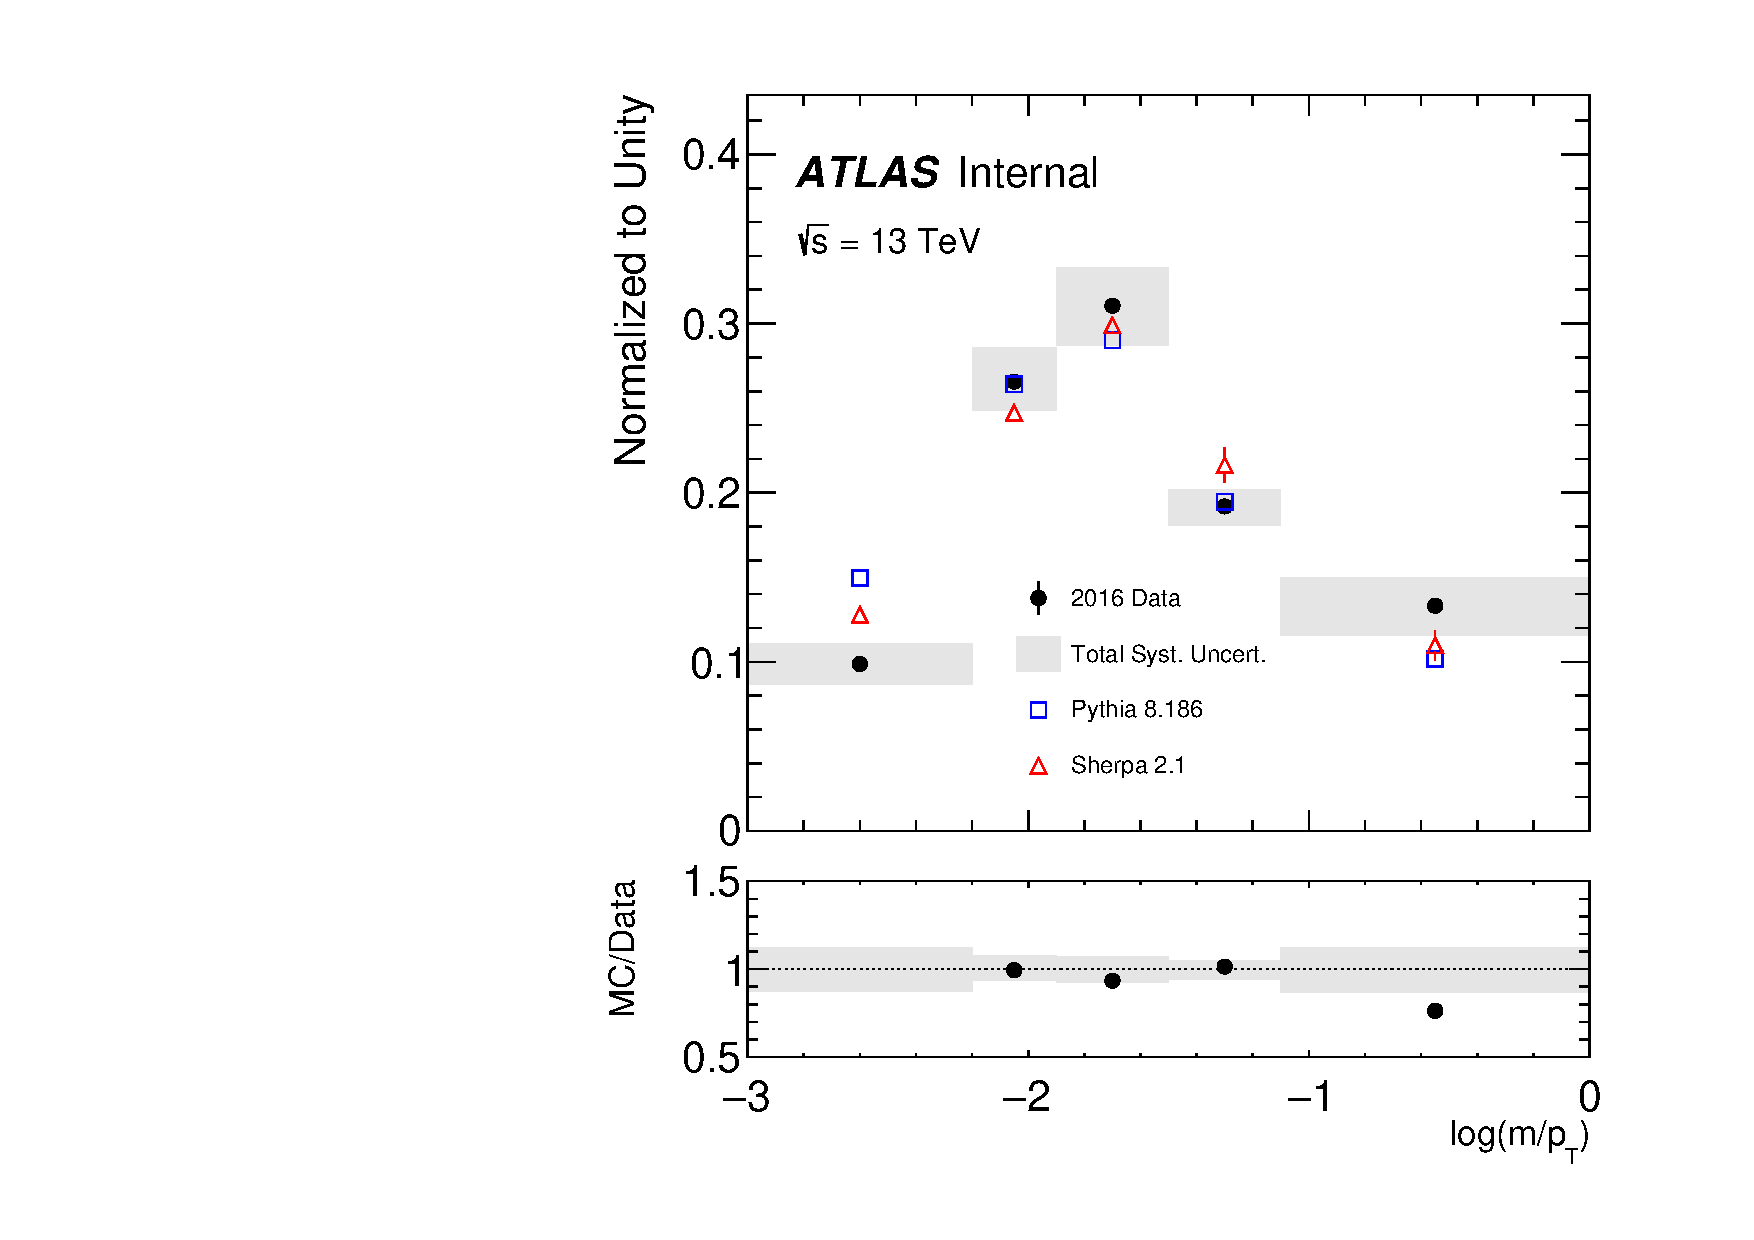
\includegraphics[width=0.45\linewidth]{figures/gbb/Unfolding/fracmasspt_unfolded_data.pdf}
\caption[]{The unfolded data compared with Pythia. The data points have error bars that are the statistical uncertainties and the bands are the total systematic uncertainties described in Sec.~\ref{sec:systs}.} 
\label{fig:gbb-results}
\end{center}
\end{figure}

\subsection{Interpretation}
\label{sec:gbb-interp}

The data will be made available through HepData so MC authors will be able to compare their models with our data at a later time.  However, it is interesting to provide some comparisons in the ATLAS paper.  Due to the large MC sizes needed for this study, we have privately produced a series of samples discussed in this section.  This setup has been extensively validated, as discussed in Appendix~\ref{sec:app-truthpreds}.  
